\documentclass{article}
\usepackage{tikz,amsmath,siunitx}
\usetikzlibrary{arrows,snakes,backgrounds,patterns,matrix,shapes,fit,calc,shadows,plotmarks}
\usepackage[graphics,tightpage,active]{preview}
\PreviewEnvironment{tikzpicture}
\PreviewEnvironment{equation}
\PreviewEnvironment{equation*}
\newlength{\imagewidth}
\newlength{\imagescale}
\pagestyle{empty}
\thispagestyle{empty}
\begin{document}
\begin{tikzpicture}[scale=0.6, every node/.style={scale=0.6}]
	\coordinate (tl) at (-1,0);
	\coordinate (bl) at (-1,-2);
	\coordinate (tr) at (10,-0);
	\coordinate (br) at (10,-2);
	\node at(4.5,-1) {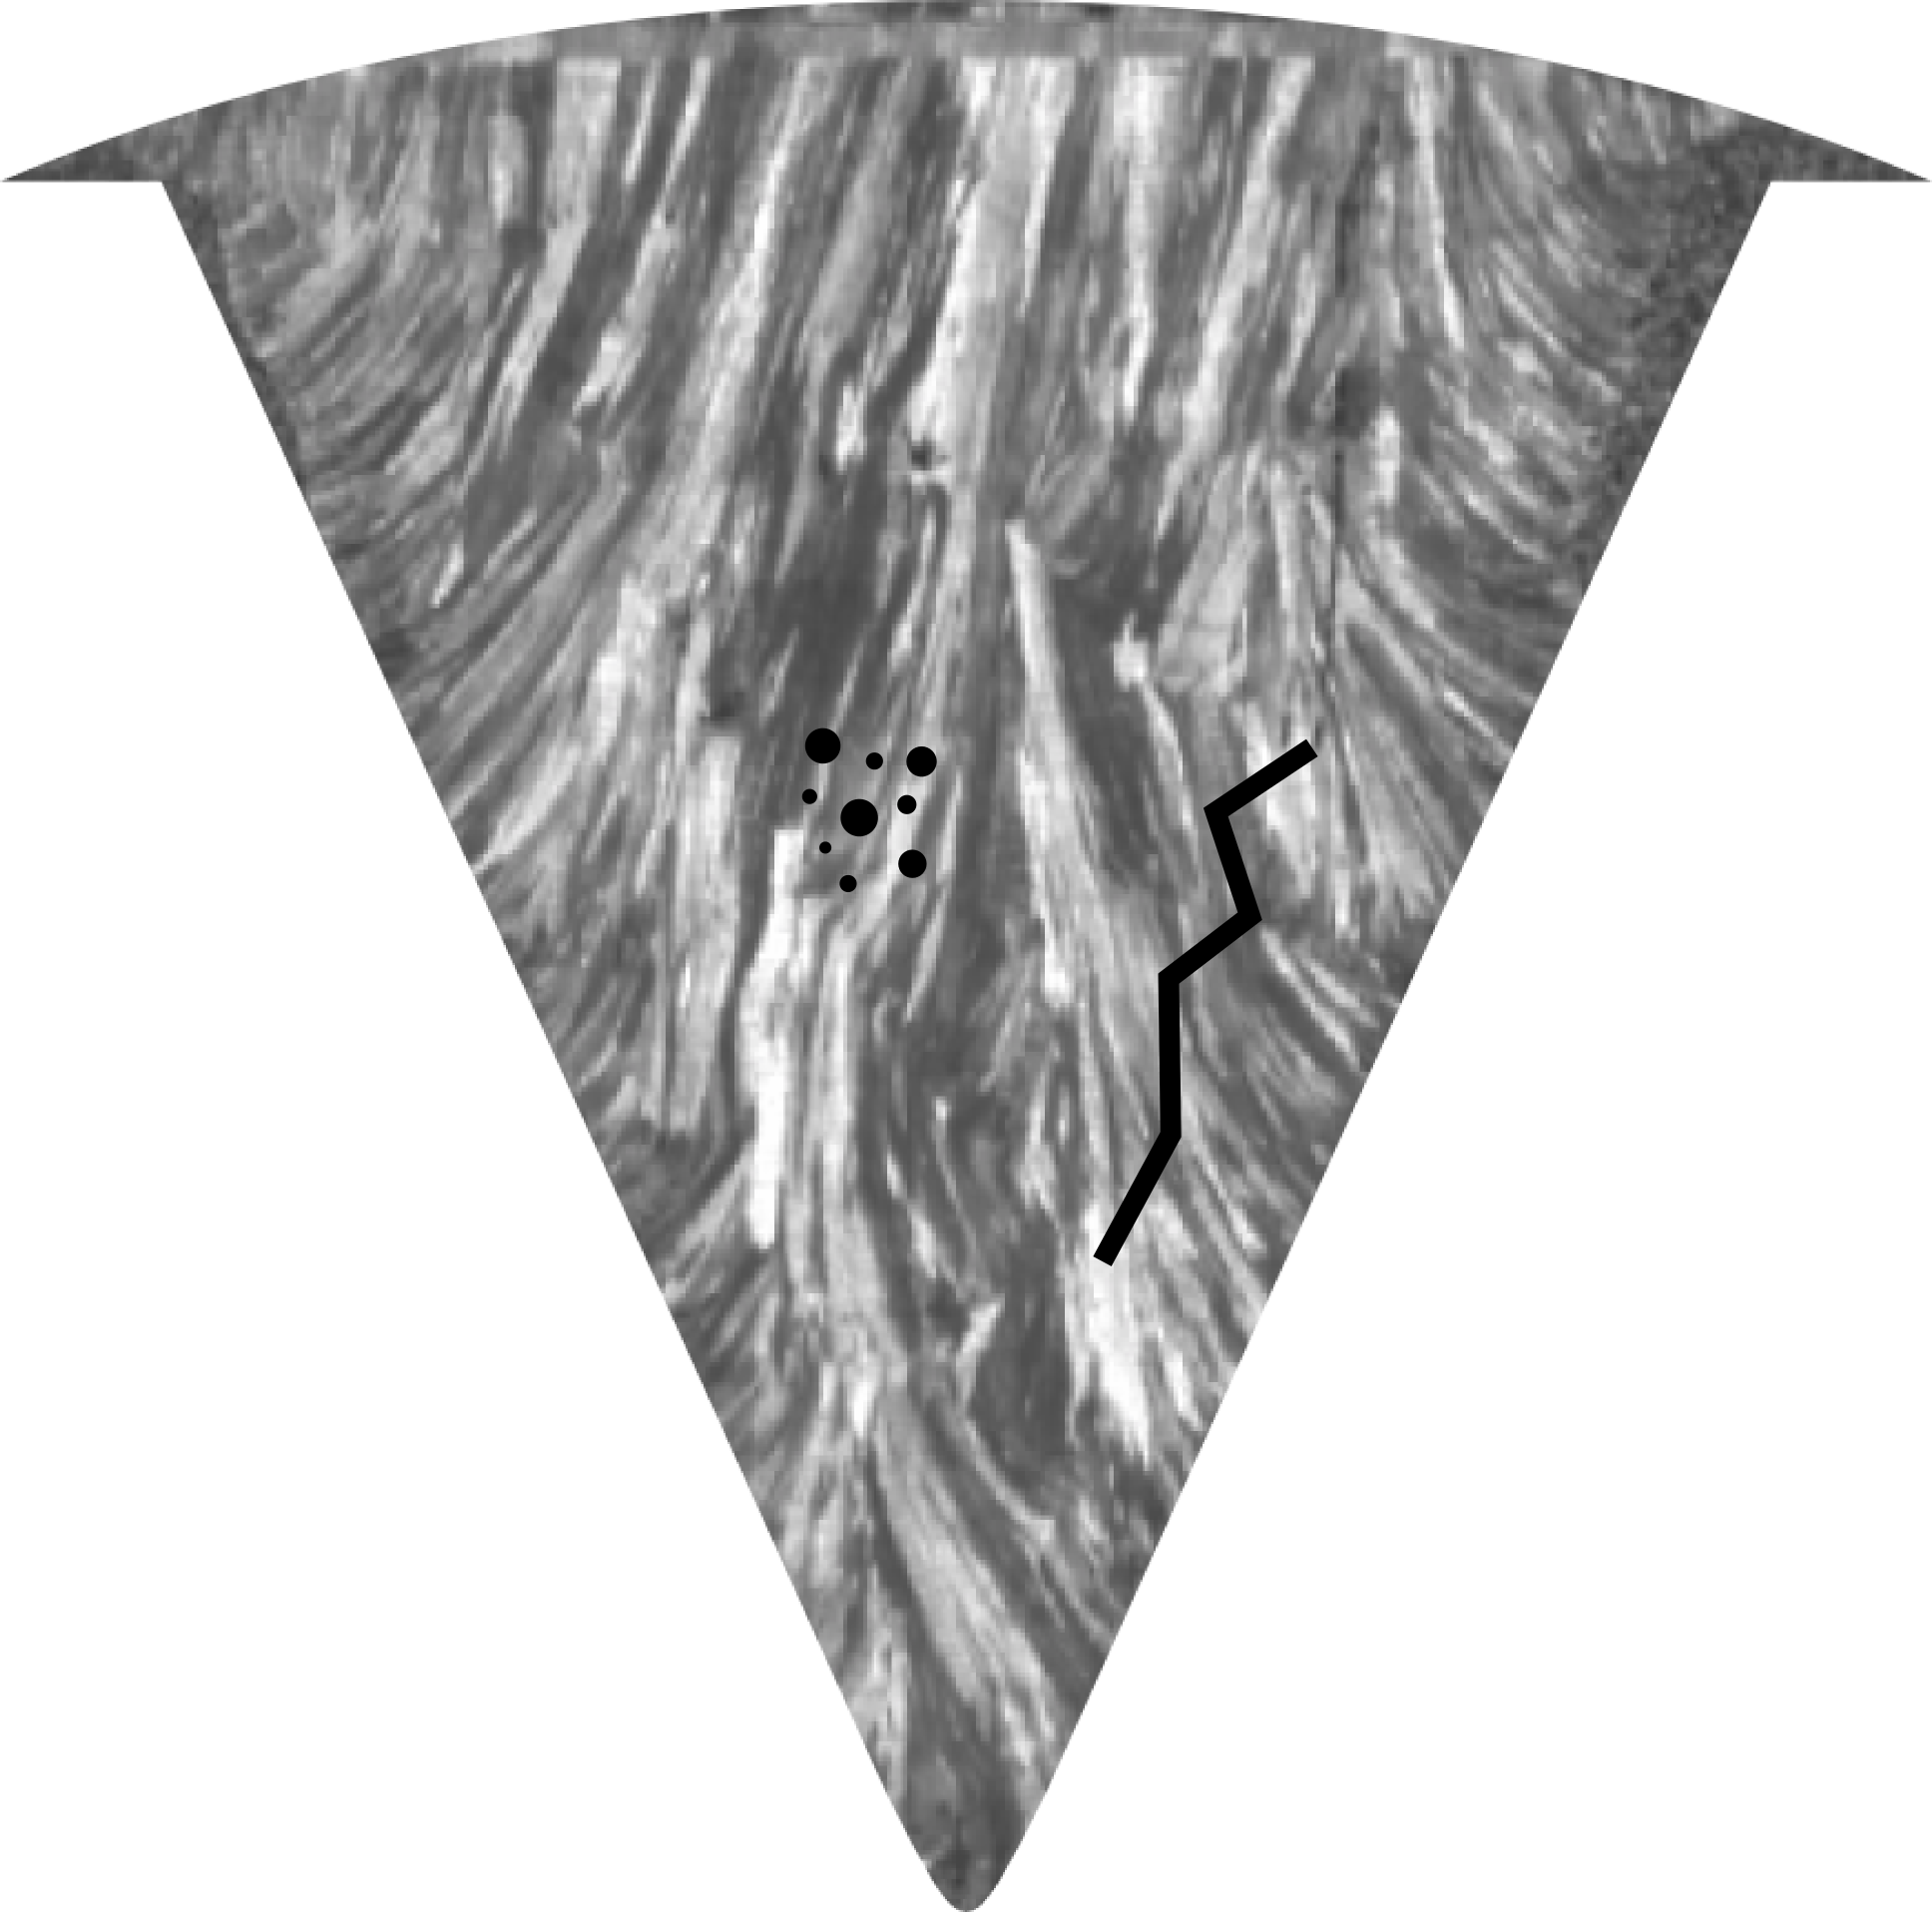
\includegraphics[scale=0.0365]{anisotrope2.png}};
	\draw [draw=none] (3.5,0) -- (4.4,-2) -- (4.6,-2) -- (5.5,0)
 			(5.7,0) .. controls (5,0.3) and (4,0.3) .. (3.3,0) 
 			(4.4,-2) .. controls (4.5,-2.2) .. (4.6,-2);
	\draw (tr)--(tl);
	\draw (bl)--(br);
	\foreach \x in {(tr) , (br)} \draw[dashed] \x -- +(1,0);
	\foreach \x in {(tl) , (bl)} \draw[dashed] \x -- +(-1,0);

		%transducteurs
	\foreach \x/\y in {3-3.2/-2.2,3-3.2/0, 6/0,6/-2.2}
		\foreach \i in {0,0.05,...,3.2} \draw (\x+\i,\y) -- +(0,0.2) (\x,\y)--(\x+3.2,\y) (\x,\y+0.2)--(\x+3.2,\y+0.2);
	\node at ($(tl)+(2.3,0.5)$) {sources/receivers};
\end{tikzpicture}
\end{document}